\uuid{aQXL}
\exo7id{7168}
\titre{exo7 7168}
\auteur{megy}
\organisation{exo7}
\datecreate{2017-07-08}
\isIndication{false}
\isCorrection{true}
\chapitre{Géométrie affine euclidienne}
\sousChapitre{Géométrie affine euclidienne du plan}

\contenu{
\texte{
% cocyclicité, bissectrice, puissance
Soit $ABC$ un triangle non isocèle en $A$. % acutangle? Pas besoin
La bissectrice intérieure $\Delta$ de $\widehat{BAC}$ coupe $[BC]$ en $A_1$ et le cercle circonscrit à $ABC$ en $A_2$.
}
\begin{enumerate}
    \item \question{Soit $D$ le symétrique de $B$ par rapport à $\Delta$. Justifier que $D \in (AC)$.}
\reponse{Par construction, la droite $\Delta$ est la hauteur et la médiane de $ABD$. Le triangle est donc isocèle en $A$ et $\Delta$ est également sa bissectrice, ce qui montre que $\widehat{BAA_1} = \widehat{A_1AD}$ et donc que $D\in (AC)$.}
    \item \question{Montrer que $A_1A_2CD$ est inscriptible.}
\reponse{Il suffit de prouver que $(A_2A_1,A_2C)=(DA_1,DC)$.
\begin{center}
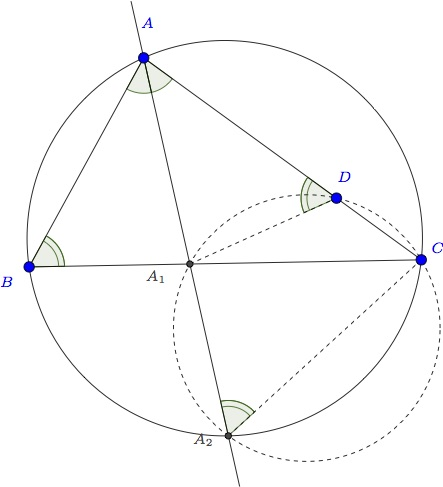
\includegraphics{../images/img007168-2}
\end{center}
Or on a :
\begin{align*}
(A_2A_1,A_2C)
&= (A_2A,A_2C)\\
&= (BA,BC) \text{ (car $ABCA_2$ est inscriptible)}\\
&= (BA,BA_1) \text{ (mêmes droites)}\\
&= (DA,DA_1) \text{ (par réflexion suivant $\Delta$)}\\
&= (DC,DA_1) \text{ (mêmes droites)},
\end{align*}
ce qu'il fallait démontrer.}
    \item \question{Montrer que $AA_1\cdot AA_2 = AB\cdot AC$. % puissance}
\reponse{Remarquons déjà que $AB=AD$.  D'autre part, il suffit de montrer que
\[ \frac{AA_1}{AD} = \frac{AC}{AA_2}.\]

La question précédente montre que les triangles $ADA_1$ et $AA_2C$ sont (inversement) semblables, puisqu'ils ont deux (et donc trois) angles en commun. Les rapports entre les côtés sont donc égaux, c'est-à-dire précisément
\[ \frac{AA_1}{AD} = \frac{AC}{AA_2}.\]

Remarque : si on connaît la notion de puissance d'un point par rapport à un cercle, on peut conclure plus vite : les deux produits égaux sont la puissance de $A$ par rapport au cercle $A_1A_2CD$.}
\end{enumerate}
}
